\documentclass[xetex,mathserif,serif]{beamer}
\usepackage{xeCJK}
\usepackage{listings}
\usepackage{hyperref}
\usepackage{algorithmic,algorithm}
\usepackage{graphicx}
\usepackage{subfigure}
\usepackage{fontspec}
\usepackage{setspace}

\usetheme{Copenhagen}
\usecolortheme{seahorse}
\useoutertheme{infolines}
\useinnertheme{rectangles}
\setmainfont{Times New Roman}

\AtBeginSection[]
{
  \begin{frame}
    \frametitle{Table of Contents}
    \tableofcontents[currentsection]
  \end{frame}
}
\AtBeginSubsection[]
{
  \begin{frame}
    \frametitle{Table of Contents}
    \tableofcontents[currentsection,currentsubsection]
  \end{frame}
}

\begin{document}
\title[Weekly report] % (optional, only for long titles)
{Sequence Classification(序列分类)}
\subtitle{Real value sequence as exemplified}
\author{刘精昌 } % (optional, for multiple authors)
\date{\today}
\subject{Weekly report}

\begin{frame}
\titlepage
\end{frame}

\section{introductions to sequence and sequence classification}

\begin{frame}
\frametitle{sequence}
\begin{exampleblock}{what is sequence?}
\begin{itemize}
  \item DNA and protein sequence
  \item The time series of heart rates
  \item Trend of stock
\end{itemize}
\end{exampleblock}

\begin{block}{How to represent sequence?}
\begin{itemize}
  \item An ordered list of the symbols,\ such as ACCCCCGT
  \item A sequence of real values,\ such as 0.1,0.3,0.5,0.1,...
\end{itemize}
\end{block}
\end{frame}

\begin{frame}
\frametitle{sequence classification}
\begin{exampleblock}{Applications of sequence classification}
\begin{itemize}
  \item gait analysis
  \item speech recognition
  \item learn the functions of a new protein
\end{itemize}
\end{exampleblock}
\pause
\begin{block}{task}
A sequence may carry a class label. Given $L$ as a set class labels,\ the task of $(conventional) \; sequence \; classification$ is to learn a $sequence \; classifier \; C$, which is a function mapping a sequence $s$ to a class label $l \in L$,written as,\[C:s \to l,l \in L\]
\end{block}
\end{frame}

\begin{frame}
\frametitle{methods and problems}
\begin{block}{methods}
$1$NN,\ 待分类序列的label即距离其最近的序列的label
\end{block}
\hspace{15em}
\begin{block}{problems}
How to measure the distance between two sequence?
\end{block}
\end{frame}

\section{Dynamic Time Warping(DTW)}
\subsection{Why is DTW?}
\begin{frame}
% \frametitle{}
\begin{block}{Euclid distance}
The simplest distance is Euclid distance:
\[dist\left( {s,{s^{'}}} \right) = \sqrt {\sum\limits_{i = 1}^L {{{\left( {s\left[ i \right] - {s^{'}}\left[ i \right]} \right)}^2}} } \]
And other similar distance.
\end{block}
\end{frame}

\begin{frame}
\frametitle{Weakness of Euclid distance}
\begin{spacing}{1.5}
\begin{itemize}
  \item 需要满足两序列长度相同。
  \item 设想这样一种情况。在步态分析中,同一测试者的步速可能不同,或者在某时间段上存在着加速和减速。那么对于其两段步态序列,比较相似的步态之间可能会有一定的时间差,而上面的这些距离测度只会将同一时刻的步态相比较。也就是说,上面的这些距离测度不能反映出序列比较中的错位。
\end{itemize}
\end{spacing}
\end{frame}

\begin{frame}
\begin{figure}
  \centering
  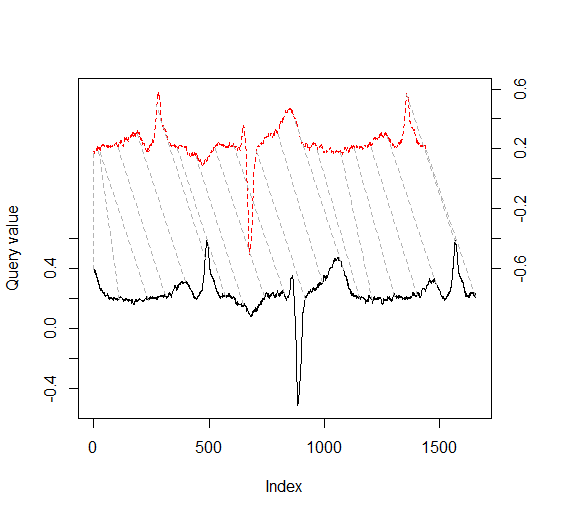
\includegraphics[width=0.65\textwidth]{two_way_plot.png}
  \caption{DTW示意图}\label{fig:1}
\end{figure}
\end{frame}

\subsection{How to compute DTW}
\begin{frame}
\frametitle{Definitions}
\begin{itemize}
  \item $Q = q_1,q_2,\cdots,q_i,\cdots,q_m$,\ $C = c_1,c_2,\cdots,c_j,\cdots,c_n$
  \item $D(i^{th},j^{th}) = d(q_i,c_j) = (q_i - c_j)^2$
  \item warping path: \ \[W = w_1,w_2,\cdots,w_k,\cdots,w_K \quad max(m,n) \le K \le m+n-1 \]
  $w_k = (i,j)_k$
\end{itemize}
\end{frame}

\begin{frame}
\begin{figure}
  \centering
  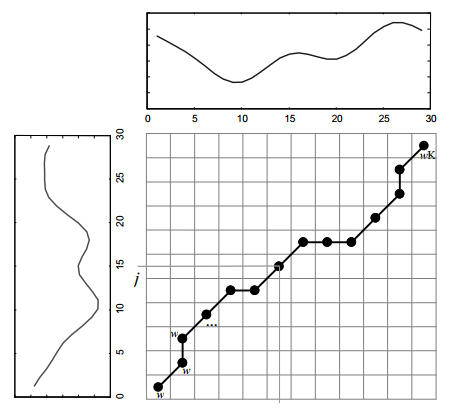
\includegraphics[width=.65\textwidth]{three_way_plot.png}
  \caption{warping path 示意图}\label{fig:2}
\end{figure}
\end{frame}

\begin{frame}
\frametitle{Constraints}
\begin{spacing}{1.2}
\begin{itemize}
  \item{\textbf{Boundary conditions: }}$w_1 = (1,1)$ and $w_K = (m,n)$
  \item{\textbf{Continuity: }}Given $w_k = (a,b)$ then $w_{k-1} = (a^{'},b^{'})$ where $a-a^{'} \le 1$ and $b-b^{'} \le 1$
  \item{\textbf{Monotonicity: }}Given $w_k = (a,b)$ then $w_{k-1} = (a^{'},b^{'})$ where $a-a^{'} \ge 0$ and $b-b^{'} \ge 0$
\end{itemize}
\end{spacing}
\end{frame}

\algsetup{linenosize = \tiny,
    linenodelimiter=.}
\begin{algorithm}
\caption{Calculate DTW}
\begin{algorithmic}[1]
\small
\REQUIRE $s:array[1..m], t:array[1..n]$
\ENSURE $DTW[m,n]$

\STATE $DTW := [0..m,0..n]$
\FOR{$i:=0$ to $m$}
\STATE $DTW[i,0] := inf$
\ENDFOR
\FOR{$j:=0$ to $n$}
\STATE $DTW[0,j] := inf$
\ENDFOR
\STATE $DTW[0,0] := 0$
\STATE
\FOR{$i:=$ $1$ to $m$}
\FOR{$j:=$ $1$ to $n$}
\STATE $cost:=d(s[i],t[j])$
\STATE $DTW[i,j]:=cost+min(DTW[i-1,j],DTW[i,j-1],DTW[i-1,j-1])$
\ENDFOR
\ENDFOR
\end{algorithmic}
\end{algorithm}

\begin{frame}
\frametitle{target and evaluation}
\begin{block}{Target}
minimizes the warping cost:
\[DTW\left( W \right) = \sum\limits_{k = 1}^K {d\left( {{w_{ki}},{w_{kj}}} \right)} \]
${d\left( {{w_{ki}},{w_{kj}}} \right)}$ :\  the distance between two data point indexes(one from $Q$ and one from $C$) in the $k^{th}$ element of the warp path.
\end{block}

\begin{block}{Evaluation}
$\gamma(i,j)$: cumulative distance
\[\gamma \left( {i,j} \right) = d\left( {{q_i},{c_j}} \right) + \min \left( {\gamma \left( {i - 1,j} \right),\gamma \left( {i,j - 1} \right),\gamma \left( {i - 1,j - 1} \right)} \right)\]
\end{block}
\end{frame}

\begin{frame}
\frametitle{Trace back the best path}
\begin{figure}
  \centering
  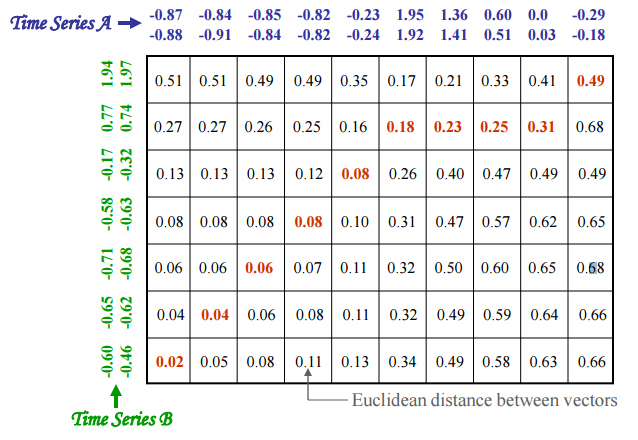
\includegraphics[width=0.7\textwidth]{trace_back.png}
  \caption{\centering A greedy search is performed that evaluates cells to the left,down,and diagonally to the bottom-left}\label{fig:3}
\end{figure}
\end{frame}

\subsection{Speed up the DTW calculations}

\algsetup{linenosize = \tiny,
    linenodelimiter=.}
\begin{algorithm}
\caption{Calculate DTW with warp window}
\begin{algorithmic}[1]
\small
\REQUIRE $s:array[1..n], t:array[1..m]$, $w:$warp window
\ENSURE $DTW[n,m]$
\STATE $DTW := array[0..n,0..m]$
\STATE $w := max(w,\left| {n-m} \right|)$

\FOR {$i := 0$ to $n$}
\FOR {$j := 0$ to $m$}
\STATE $DTW[i,j] := inf$
\ENDFOR
\ENDFOR
\STATE $DTW[0,0] := 0$
\STATE
\FOR {$i := 1$ to $n$}
\FOR {$j := max(1,i-w)$ to $min(m,i+w)$}
\STATE $cost := d(s[i],t[j])$
\STATE $DTW[i,j]:=cost+min(DTW[i-1,j],DTW[i,j-1],DTW[i-1,j-1])$
\ENDFOR
\ENDFOR
\end{algorithmic}
\end{algorithm}

\begin{frame}
\frametitle{warp window}
\begin{itemize}
  \item An obvious observation is that an intuitive alignment path is unlikely to drift/very far from the diagonal
      \vspace{1em}
    \begin{figure}
      \centering
      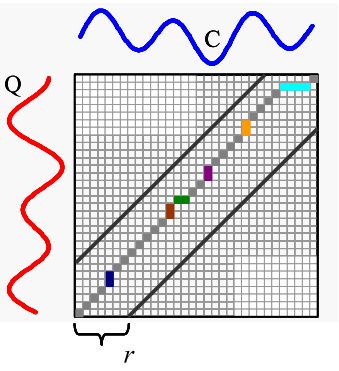
\includegraphics[width=0.35\textwidth]{warp_window.png}
      \caption{warp window}\label{fig:4}
    \end{figure}
\end{itemize}
\end{frame}

\begin{frame}
\frametitle{Piecewise aggregate representation}
\begin{figure}
    \centering
    \subfigure[原始DTW对齐]{
    \begin{minipage}[b]{0.8\textwidth}
    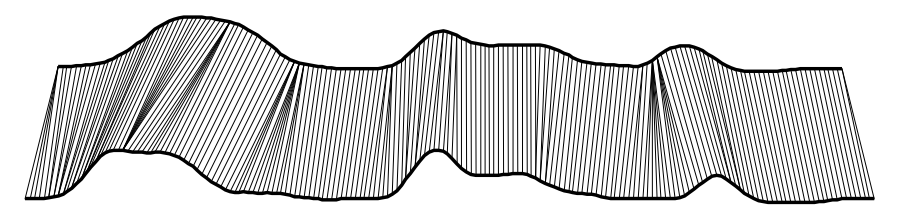
\includegraphics[width=1\textwidth]{original.PNG}
    \end{minipage}
    }
    \subfigure[PAR处理后的DTW对齐]{
    \begin{minipage}[b]{0.8\textwidth}
    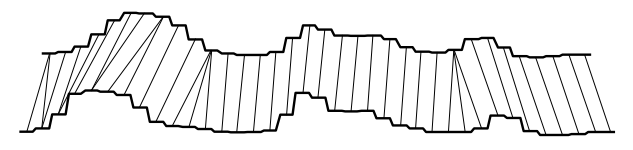
\includegraphics[width=1\textwidth]{new.PNG}
    \end{minipage}
    }
    \caption{PAR处理示意图} \label{fig:6}
\end{figure}
\end{frame}

\begin{frame}
\frametitle{FastDTW}
\begin{block}{Time and Space Complexity}
\begin{itemize}
  \item \textbf{DTW:}$O(n^2)$
  \item \textbf{FastDTW:}$O(n)$
\end{itemize}
\end{block}

\begin{exampleblock}{Three key operations}
\begin{enumerate}
  \item Coarsening(粗化)
  \item Projection(投影)
  \item Refinement
\end{enumerate}
\end{exampleblock}
\end{frame}

\begin{frame}
\frametitle{FastDTW}
\begin{figure}
  \centering
  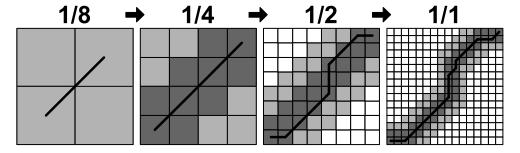
\includegraphics[width=0.8\textwidth]{FastDTW.png}
  \caption{FastDTW示意图}\label{fig:7}
\end{figure}
\end{frame}

\begin{frame}
\frametitle{Time Complexity of FastDTW}
\begin{figure}
  \centering
  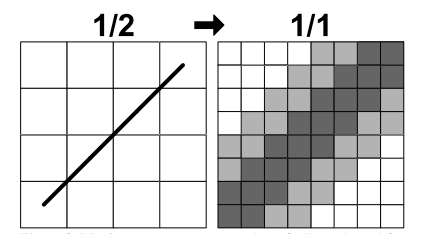
\includegraphics[width=0.4\textwidth]{evaluation.png}
  \caption{\tiny Maximum number of cells evaluated for a radius of 1}\label{fig:8}
\end{figure}

maximum number of cells\ :\ $3N+2*(2Nr) = N(4r+3)$
\newline
\textbf{\emph{Total number of cells filled: }}\[N\left( {4r + 3} \right) + \frac{N}{2}\left( {4r + 3} \right) + \frac{N}{{{2^2}}}\left( {4r + 3} \right) +  \cdots  = 2N\left( {4r + 3} \right)\]
\end{frame}

\begin{frame}
\frametitle{Time Complexity of FastDTW}
\begin{block}{Time Complexity}
\begin{enumerate}
  \item number of cells calculated:\ $2N(4r+3)$
  \item creat the coarser resolutions:\ $4N$
  \item determining the warp path by tracing throungth the matrix:\ $4N$
\end{enumerate}
\end{block}

\begin{block}{\textbf{\emph{Total FastDTW time complexity}}}
\[N(8r+14)\]
\end{block}
\end{frame}

\begin{frame}
\frametitle{Space Complexity of FastDTW}
\begin{block}{Space Complexity}
\begin{enumerate}
  \item Space of resolutions:\ $4N$
  \item Space of distance matrix:\ $N(4r+3)$
  \item Space complexity of storing the warp path:\ $4N$
\end{enumerate}
\end{block}

\begin{block}{\textbf{\emph{Total FastDTW space complexity}}}
\[N(4r+11)\]
\end{block}
\end{frame}

\subsection{experimental result}

\begin{frame}
\frametitle{experimental result}
\textbf{data:}\ 在一段间隔上加上随机误差而产生
\begin{figure}
  \centering
  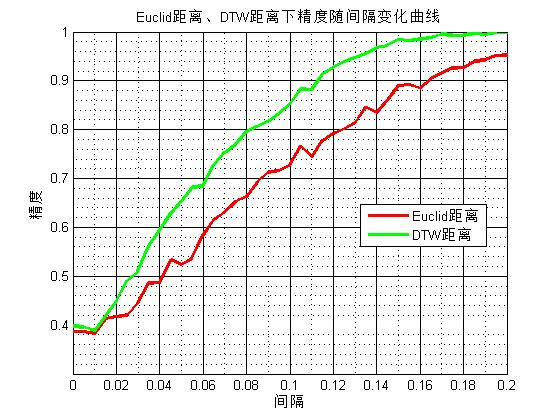
\includegraphics[width=0.6\textwidth]{interval.jpg}
  \caption{Euclid、DTW距离下分类精确度随间隔变化曲线}\label{fig:8}
\end{figure}
\end{frame}

\begin{frame}
\small
\frametitle{experimental result}
\href{http://www.cs.ucr.edu/~eamonn/time_series_data/}{TSDMA}数据集
    \begin{center}
      \begin{tabular}{|c|c|c|c|c|c|c|c|}
      \hline
      % after \\: \hline or \cline{col1-col2} \cline{col3-col4} ...
      name & Computers & Trace & FaceFour & WordsSynonyms\\
      \hline
      lasses & 2 & 4 & 4 & 25  \\
      \hline
      training set size & 250 & 100 & 24 & 267  \\
      \hline
      test set size & 250 & 100 & 88 & 638  \\
      \hline
      sequence length & 720 & 275 & 350 & 270  \\
      \hline
      error rate (Euclid) & 0.424 & 0.24 & 0.21591 & 0.38245 \\
      \hline
      error rate (DTW) & 0.332 & 0.01 & 0.15909 & 0.32445  \\
      \hline
    \end{tabular}
    \end{center}
\end{frame}

\begin{frame}
\centering
\frametitle{experimental result}
\begin{flushleft}
  \href{http://www.cs.ucr.edu/~eamonn/time_series_data/}{TSDMA}数据集
\end{flushleft}
    \begin{center}
      \begin{tabular}{|c|c|c|c|c|c|c|c|}
      \hline
      % after \\: \hline or \cline{col1-col2} \cline{col3-col4} ...
      name & Gun\_Point & Plane & StrawBerry \\
      \hline
      lasses & 2 & 7 & 2 \\
      \hline
      training set size  & 50 & 105 & 370 \\
      \hline
      test set size  & 150 & 105 & 613 \\
      \hline
      sequence length & 150 & 144 & 235 \\
      \hline
      error rate (Euclid) & 0.086667 & 0.038095 & 0.06199 \\
      \hline
      error rate (DTW) & 0.12 & 0 & 0.066884 \\
      \hline
    \end{tabular}
    \end{center}
\end{frame}

\begin{frame}
\frametitle{experimental result}
\begin{figure}[ht]
    \centering
    \subfigure[gun point]{%
    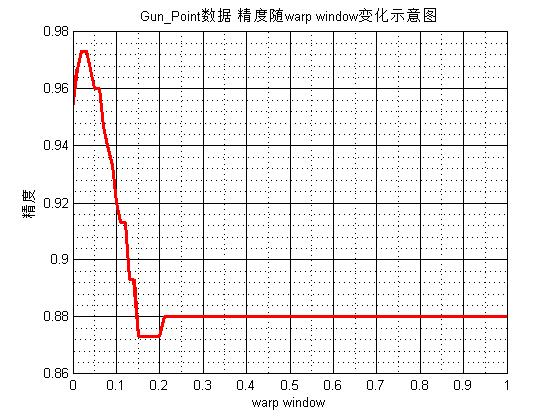
\includegraphics[width=0.28\textwidth]{gun_point.jpg}
    \label{fig:subfigure4}}
    %
    \quad
    \subfigure[WordsSunonyms]{%
    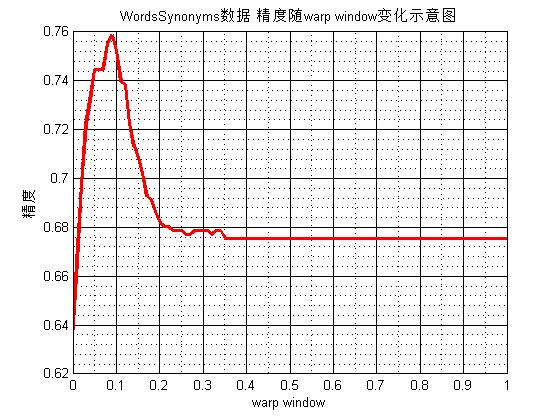
\includegraphics[width=0.28\textwidth]{WordsSunonyms.jpg}
    \label{fig:subfigure2}}
    \subfigure[facefour]{%
    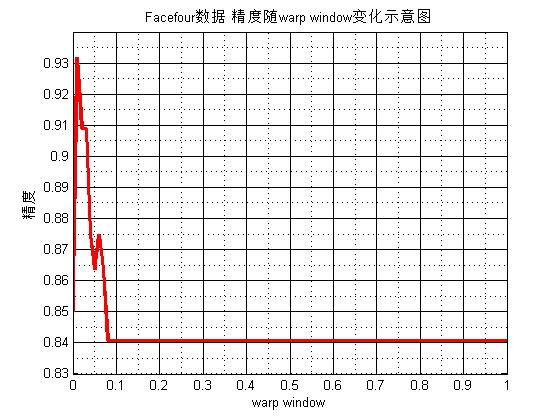
\includegraphics[width=0.28\textwidth]{facefour.jpg}
    \label{fig:subfigure3}}
    \quad
    \subfigure[interval:0.135]{%
    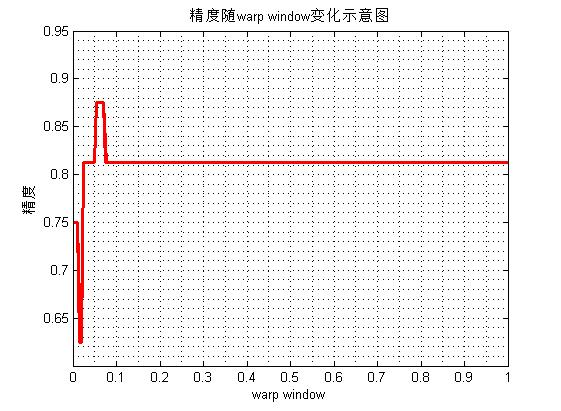
\includegraphics[width=0.28\textwidth]{accuracy_warp_window.jpg}
    \label{fig:subfigure1}}
    \caption{精度随warp window变化示意图}
    \label{fig:9}
\end{figure}
\end{frame}

\section{Shapelets}
\subsection{What is shapelets?}
\begin{frame}
\frametitle{Introdiction}
\begin{figure}
  \centering
  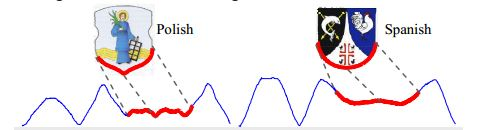
\includegraphics[width=0.6\textwidth]{shapelets.png}
  \caption{\centering shapelets are subsequences which are in some sense maximally representative of a class}\label{fig:9}
\end{figure}
\begin{block}{Advantages}
\begin{enumerate}
  \item Provide interpretable results
  \item More accuracy/robust on some datasets
  \item Faster,$O(ml)$,\ $m:$length of query sequence,\ $l:$length of shapelets
\end{enumerate}
\end{block}
\end{frame}

\begin{frame}
\frametitle{Definition}
\textbf{$SubsequenceDist(T,S) ={min}({Dist}(S^{'},S))$, for $S^{'} \in S_T^{\left| S \right|}$}
\newline
\newline
\emph{Optimal Split Point(OSP) }.\ A sequence dataset \textbf{D} consists of two classes,\emph{A} and \emph{B}.For a shapelet candidate \emph{S},we choose some distance threshold $d_{th}$ and split \textbf{D} into \textbf{$D_1$} and \textbf{$D_2$},such that for every time series object $T_{1,j}$ in \textbf{$D_1$},$SubsequenceDist(T_{1,i},S)<d_{th}$ and for every time series object $T_{2,i}$ in \textbf{$D_2$},$SubsequenceDist(T_{2,i},S)>d_{th}$. An Optimal Split Point is a distance threshold that
\[{Gain}\left( {S,{d_{{OSP}\left( {D,S} \right)}}} \right) \ge {Gain}\left( {S,d_{th}^{'}} \right)\]
for any other distance threshold $d_{th}^{'}$.
\end{frame}

\begin{frame}
\frametitle{Definition}
\emph{Shapelet. }\ Given a time series dataset \textbf{D} which consists of two classes,\ \emph{A} and \emph{B},\emph{shapelet}\textbf{$D$} is a subsequence that,\ with its corresponding optimal split point,
\[Gain\left( {shapelet\left( D \right),{d_{OSP\left( {D,shapelet\left( D \right)} \right)}}} \right) \ge Gain\left( {S,{d_{OSP\left( {D,S} \right)}}} \right)\]
for any other subsequence \textbf{$S$}.
\end{frame}

\algsetup{linenosize = \tiny,
    linenodelimiter=.}
\begin{algorithm}
\caption{Brute force algorithm for finding shapelet}
\begin{algorithmic}[1]
\small
\REQUIRE dataset \textbf{$D$},\emph{MAXLEN},\emph{MINLEN}
\ENSURE bsf\_shapelet

\STATE candidates := GenerateCandidates(\textbf{$D$},\emph{MAXLEN},\emph{MINLEN})
\STATE bsf\_gain := 0
\FOR { S in candidates}
\STATE gain:=CheckCandidate(D,S)
\IF {gain>bsf\_gain}
\STATE bsf\_gain :=gain
\STATE bsf\_shapelet :=S
\ENDIF
\ENDFOR
\end{algorithmic}
\end{algorithm}

\subsection{Find and speed the shapelet}

\begin{frame}
\frametitle{Speedup methods}
\begin{block}{Subsequence Distance Early Abandon}
\begin{itemize}
  \item Stop distance calculations once the partial distance exceeds the minimum distance known so far.
\end{itemize}
\end{block}

\begin{figure}
  \centering
  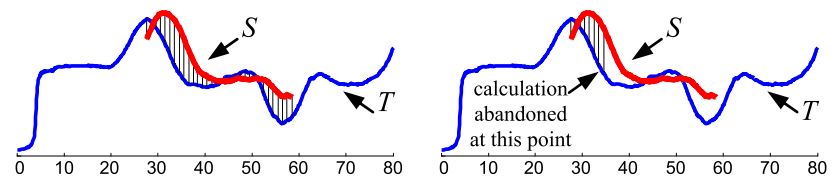
\includegraphics[width=0.65\textwidth]{subdistance.png}
  \caption{Subsequence Distance Early Abandon}\label{fig:9}
\end{figure}
\end{frame}

\begin{frame}
\frametitle{Admissible Entropy Pruning}
\begin{figure}
    \centering
    \subfigure[\footnotesize 排序依照数据集序列到候选序列距离,并计算当前的信息增益]{
    \begin{minipage}[b]{0.8\textwidth}
    \centering
    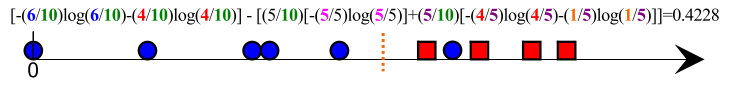
\includegraphics[width=0.8\textwidth]{Entropy1.PNG}
    \end{minipage}
    }
    \subfigure[\footnotesize 已计算了数据集中的五个序列到候选序列的距离]{
    \begin{minipage}[b]{0.8\textwidth}
    \centering
    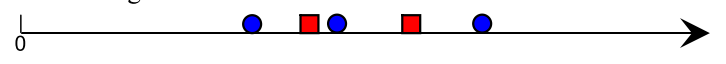
\includegraphics[width=0.8\textwidth]{Entropy2.PNG}
    \end{minipage}
    }
    \subfigure[\footnotesize 数据集剩余序列使得信息增益最大的极端位置]{
    \begin{minipage}[b]{0.8\textwidth}
    \centering
    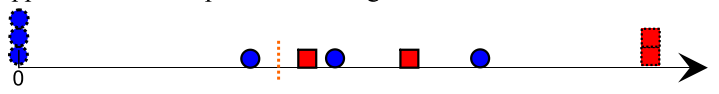
\includegraphics[width=0.8\textwidth]{Entropy3.PNG}
    \end{minipage}
    }
    \caption{Entropy Prunning 示意图} \label{fig:10}
\end{figure}
\end{frame}

\begin{frame}
\begin{center}
  \Huge{Q \& A}
\end{center}
\end{frame}

\begin{frame}
\begin{center}
  \Huge{谢谢观看}
\end{center}
\end{frame}
\end{document}
